\documentclass[a4paper, 10pt]{extarticle}
\usepackage[a4paper , top=36mm, right=36mm,left=36mm, bottom=36mm]{geometry}
\usepackage{graphicx}
\graphicspath{{assets/images/}}
\usepackage{float}
\usepackage{amsmath}
\usepackage{amssymb}
\usepackage[pdftex,
pdfauthor={Joby Reuben, Purva Chaudhari},
pdftitle={Bitcoin Blink : A Peer-to-Peer Global Finance System},
pdfkeywords={Bitcoin, Bitcoin Hard fork, Bitcoin blink, Proof of Speed, Scalable consensus, Cryptocurrency, Tokenization, Blockchain}]{hyperref}
\usepackage{xurl}
\usepackage{amsfonts} 
\usepackage[font=footnotesize,labelfont=bf]{caption}
\usepackage{indentfirst}
\renewcommand{\abstractname}{\vspace{-\baselineskip}}
\setlength{\belowcaptionskip}{-10pt}
\font\myfontt=cmr12 at 9pt
\usepackage{color}
\usepackage{comment}
\title{
 \large \textbf{Bitcoin Blink : A Peer-to-Peer Global Finance System}
\author{ \myfontt Joby Reuben \\ \myfontt joby@bitcoinblink.org \and  \myfontt Purva Chaudhari \\ \myfontt purva@bitcoinblink.org \and \myfontt Ajay Joshua \\ \myfontt ajay@bitcoinblink.org}}
\date{}
\begin{document}
\maketitle
\begin{abstract}
\noindent \textbf{Abstract.} Bitcoin's Proof-of-Work consensus is replaced with a propagation competition on blocks sent across a certain set of validators under a time interval stamped with cryptographic proofs to claim fees and solve forks as per proof weight. To achieve adaptable scalability, each block's size is determined in consensus among elected nodes to reduce transaction waiting time. Gossip systems are replaced with a privacy-centered direct messaging system by constructing encrypted paths to deliver unconfirmed transactions and confirmed blocks. Apart from bringing speed, we resolved the need for a single transaction fee token by bringing forth a novel non-custodial per-token staking system to allow users to pay transaction fees in any token. The ``bitcoin" as a currency will ensure network security with staking and yielding fees. Since Bitcoin script adapts a Turing-incomplete language, fees are imposed for renting UTXOs which makes transactions cheaper and optimizes the chain's ledger size. We propose solutions for regulation revolving around taxation within the self-custody ecosystem by offloading responsibilities to wallet providers. 
\end{abstract}
\section{Introduction}
The Bitcoin Network \cite{nakamoto2008bitcoin} and other altcoin blockchains with newer consensus and programmable money are unable to compete with centralized payment providers in speed and volume due to their sheer inability to scale with centralization issues. Many consensus models rely on external validation concepts such as finding a nonce and proving stake instead of rules tied to propagation itself. Imposing heavy reliance on users to acquire native chain tokens diminishes the adoption of blockchain, thus keeping them far from the wonders of this technology. Decentralized networks can effectively adapt to users’ needs by 1. Increasing block size 2. Decreasing block time 3. Eliminating low-efficient nodes 4. Increasing the requirement for node joining 5. Choosing producers by performance. Retail staking with non-custodial solutions encourages users to stake their bitcoin to become a world reserve currency for ensuring the security of every financial instrument.

Instead of storing UTXOs for an indefinite period, which compromises storage, renting UTXOs and replacing them with a fingerprint after they have expired without altering the block’s Merkle-root provides cheaper fees. Bitcoin’s unlocking script offers developers to create custom scripts with regulatory options involving various types of taxes within its UTXOs, performing identity verification off-chain, with signatures instructing nodes to validate regulated payments under self-custody of tokens. Decentralized Altcoins can be bridged one way to facilitate payments inside a scalable decentralized infrastructure. A floating rate stable coin \cite{stablecoin} without pegging to fiat can be issued with bitcoin as collateral for staking and yielding fees in the future. Basic banking solutions can be developed in Bitcoin script, whereas common computable programs can be deployed to a Layer 2 State Machine \cite{wood2014ethereum}, where nodes update the state by providing a Proof-of-Receipt paid in any token in the Bitcoin network.
\section{Bitcoin Blink} 
\subsection{Validation}
Block size denotes the amount of data that can be propagated across every node on the Bitcoin network. Hence, its success rate is directly dependent on the bandwidth each node allocates for confirmed block transmission. Block size is not limited and is fixed in every new block, which assures that every validator of the block can send and receive the data size. Variable block size helps to scale the network by increasing transactions per block when nodes upgrade and announce their bandwidth. A ZK-SNARK-based proof takes a node’s bandwidth as a public input signal, which is compared to the threshold range of the desired bandwidth of the network. To prevent tampering, the node will commit a salt, which is a large random number that will be added to the bandwidth to generate the $xyz$ hash which will be verified in the proof. Thus, the proof will attest its bandwidth output to the UTXO’s script and get validated.\\
\begin{figure}[H]
\begin{center}
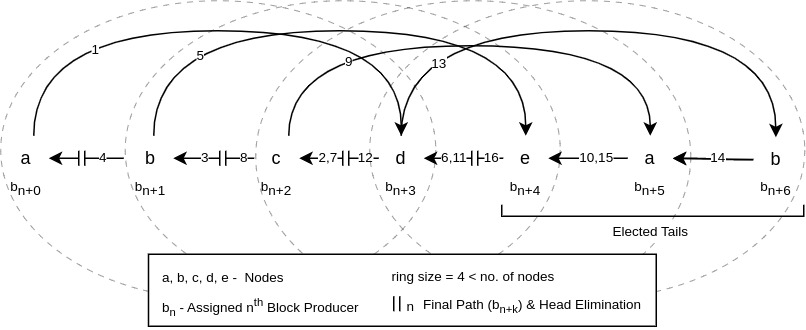
\includegraphics[width=11cm]{ring}
\end{center}
\end{figure}
The network in consensus can restrict low bandwidth nodes from participating in the election to produce blocks by keeping the election requirement variable. Bandwidth requirements are increased for nodes to get elected for the next block production can assure the capacity to hold more transactions to scale further. Elections will be conducted based on nodes' bandwidth and each node's honesty weight. Node identities are masked by their public keys encouraging privacy. For each block, the elected node will produce, and a set of nodes will validate and attach to the longest chain \cite{nakamoto2008bitcoin}. This set of nodes is finite and unique for every block and is called a ``ring validator". After each block's confirmation, the head of the ring is eliminated and a tail is elected which can be validated by nodes during propagation. The ring head after receiving the confirmed block will acquire bandwidth to gossip its block over to other full or SPV nodes to secure its rewards. The tail election's random seed is taken from concatenating Merkle-Chain-root and Hash Proof \cite{yakovenko2018solana} of the recent head's confirmed block. Thus, the election is conducted for every block where a tail node is assigned.
\subsection{Propagation}
A Block is collectively validated but constructed as snips - divisible block chunks by the producer and directly messaged to the block's ring validators with routing instructions to propagate and get confirmed. Each snip references the previous snip's hash similar to the chain of blocks for proper identification of each block's snips. For a block, a competition to deliver all snips under $x$ time interval in a finite number of hashes is required to win rewards and avoid slashing of fees. When a block fails to win, it will do an intra-block fork and not mint its last of snips which will contain the fees and rewards. Hash proofs are attached for every snip during propagation among its assigned ring validators to declare the state of each block's competition and resolve forks. Failed block fees and rewards are slashed by sending them to a burn address by the next blocks which also results in the addition of negative weights that indirectly slashes the node's bandwidth costing capital. Null-Blocks are self-minted by its ring validators with proofs.\\
\begin{figure}[H]
\begin{center}
\includegraphics[width=12cm]{Snips}
\end{center}
\end{figure}
To synchronize time, each node's single-thread hash rate per second of a specific hash function is proved cryptographically onchain and taken in multiples of a reference hash rate. An Individual hash-rate proof is provided along with bandwidth proof for every $x$ block height (ring size) before it expires which trustlessly synchronizes all nodes as a single hardware producing continuous hashes concated with all snips. The ZK IHR proofs are algorithmically similar to the bandwidth proofs, where the hash rate provided by the node is compared to the threshold range of the desired hash rate and salt is used to prevent tampering attacks. This time-based competition can be termed ``Proof of Speed".
\subsection{Forks}
\begin{figure}[h]
\begin{center}
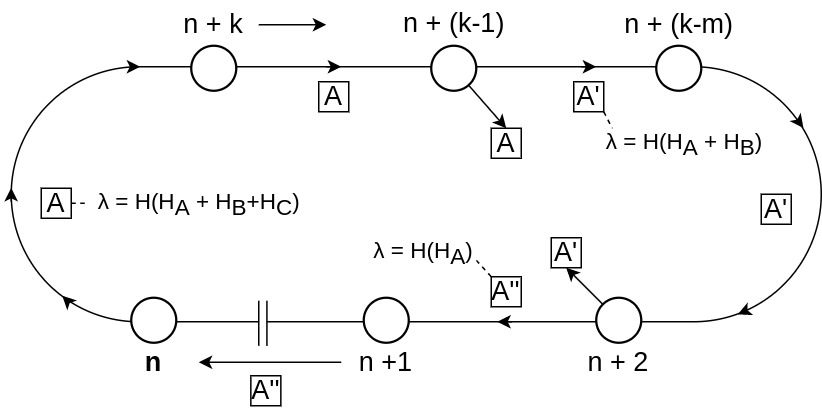
\includegraphics[width=9cm]{intrafork}
\end{center}
\end{figure}
Confirmed blocks as snips are streamed in a backward ring manner (block$_n$ to block$_{n+k}$...block$_{n+1}$). For each block to prove block time by providing Hash proofs, a set of validators is initialized by the ring's size denoting the unique number of blocks and their producers. Intra-block forks arise when ring validators reject snips of a block which can be resolved by the very next block providing instant finality to users. Intra-block forks can be minimized by keeping the ring size variable and always lesser than the total number of nodes, a viable alternative to sharding. Block size and time are decided on consensus by the block's ring validators bringing a healthy propagation. Bandwidth upgrades are needed for the nodes which initiate the intra-block fork and are punished by the network by imposing negative weights. Each new block will include the previous block's Hash proof which resolves the intra-block forks by verifying the accepted snips and updating the chain using Merkle Chain Roots. During the offline activity of ring validators, Inter-block forks arise which can be resolved by attesting Hash Proofs of offline activity and thereby adding negative weights to it. Hence, each block will have its ring validators who are assigned by onchain accounted bandwidth and honesty weights, where the heaviest Hash-proofed version of the block$_n$ is added to the longest chain.
\subsection{Messaging}
Delivery of unconfirmed transactions to nodes plays an important role in finality. Shared mempools defile the network with duplicated data, resulting in a poor choice of transactions by accepting higher fees to include in a block. A direct-messaging system should be deployed with messaging instructions specific to each party as opposed to gossip protocols. Paths are attached with unconfirmed transactions directly from the constructed network graph, which is available to all nodes with public keys as pseudonymous identities protecting privacy. Two peering parties mutually sign a 2–2 random message for every $x$ block height (ring size) and are gossiped across the network to identify the connection as online. All the signed random messages prove that each pubkey signature can display a network topology map from a node's point of reference.
\begin{figure}[H]
\begin{center}
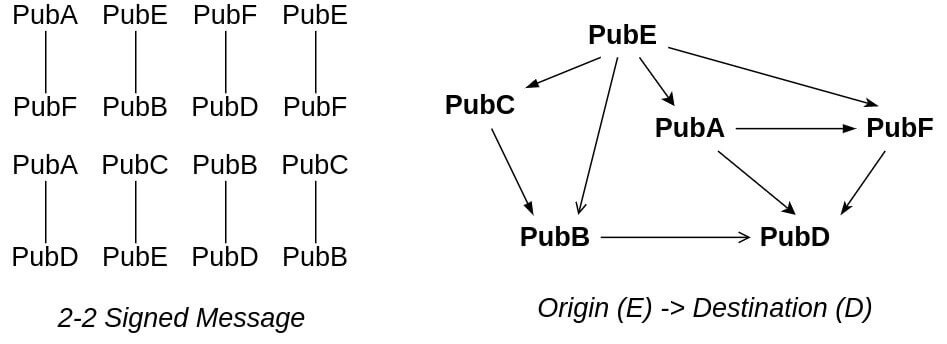
\includegraphics[width=8cm]{topology}
\end{center}
\end{figure}
Paths are encrypted end-to-end with routing \cite{poon2016bitcoin} instructions so that the origin cannot be traced. Nodes route transactions to the destinations where producers can attach the transaction to their allocated block. Since the block producers and their stake information is available in the public ledger, wallet providers can construct transactions along with path information that routes to the nearest blocks for instant finality. Transactions are always atomic, providing a solution to queuing issues. Responsibilities are provided to all participants, where nodes only receive the transactions that they need to include, and wallet providers should construct shorter paths to provide the best user experience.
\subsection{Staking}
The chain native token - bitcoin can be staked for nodes' public keys with specified token IDs, where the collateral can be used only once for a block. This results in a stake per token per block bringing the throughput (tps), per token basis. The proofs are based on Zk-Snark-based Semaphore protocol \cite{semaphore} which will allow users to prove their membership in a group and send signals without revealing the original identity. Each token per block's collateral requirement is given in bitcoin denominations. This collateral requirement provides security to restrict fraudulent tokens by requiring a bitcoin exchange rate at initial for the token's transaction to be included in the block. The bitcoin exchange rate inherent to the system independently offers market rates in a trustless manner without requiring a stable fiat-based tokens nor off-chain oracles. 

For specific nodes, bitcoins can be staked to collateralize or lock in their allocated block. Staked bitcoins can be withdrawn at any time, with no vesting period, except when the block is being created. This brings in a retail and non-custodial solution as opposed to security deposit-type PoS chains. Delegators won't lose their stakes as slashing is done directly on the fees during intra-block forks. Wallet providers can offer their general users savings wallets to avail liquidity for staking from which users can benefit from a risk-free annual percentage yield. In this way, for a specific token's transaction to be included in a block, the first of transactions should prove the collateral specific to the token.
\subsection{Renting}
Instead of a single Merkle-root for a block, each snip's Merkle-root is taken and linearly hashed to find the Merkle-Chain-root. Since snips can be rejected by validators and cannot be tampered with once it is streamed to ring validators, it is unsure to predict a Merkle-Chain-root making it a pseudo-random value. Inside a snip contains parsed transactions whose hashes are taken to find the snip's Merkle-root can be pruned if the UTXOs are spent, burnt, or expired. Each UTXO expiry block height is embedded in its script, and can be scanned by nodes, and pruned to optimize their data storage. Wallet providers can store each of their users' transaction history and can be audited onchain using Merkle-Chain-roots. Renting rates can be independently voted by producer nodes per byte per block in bitcoins. Users cannot directly pay for rent, but rather each new UTXO created is charged a transfer fee in the range of 0.05\% - 0.005\% decided based on the total volume of all transactions settled on the previous set of blocks (ring size).
\begin{figure}[H]
\begin{center}
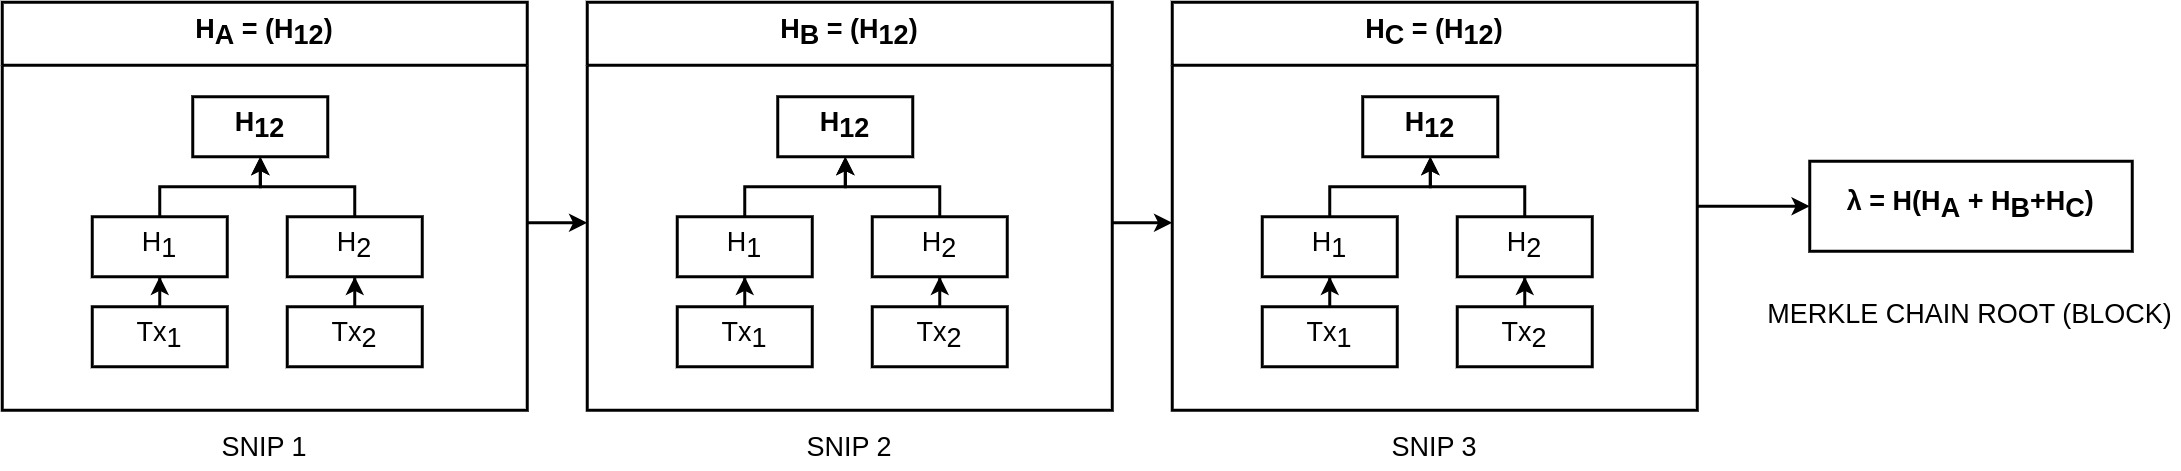
\includegraphics[width=13cm]{merklechain}
\end{center}
\end{figure}
 Transfer fee charges more fees for higher value utxos and less for lesser value utxos bringing ease to transact for retailers. Each UTXO will set an expiry date for itself. Users can be incentivized by charging zero fees to combine UTXOs to a single balance holding UTXO with an increased expiry value saving validators' disk space. 
\subsection{Rewards}
Rewards are given for each snip hash concated with transactions validated by Hash proofs. Since newly mined bitcoins for a period of time are definite and each block's time is capped in reference hash-rate, new bitcoins can be supplied exactly proportional to the current Bitcoin issuance rate with halving. The halving of Bitcoin issuance is done every $R \cdot (1.26 \cdot 10^8)$ hashes, where R is the reference single thread hash rate. Each hash proof represents work done by nodes on validating and propagating transactions. When an intra-block fork arises due to rejected snips, the rest of the block time and its allocated rewards are slashed. Meanwhile, when a block is fully minted before the block time finishes, the rest of its allocated rewards are distributed to the current halving period. This incentivizes nodes to attest and receive snips at the earliest to get an increased block reward in the upcoming block production. Tax outputs and rewards are attached as zero input transactions (coinbase tx) within the snip it contains. Fee outputs are created as a separate snip which denotes the end of a block.

During staking, producers announce their accepted tokens for which they will directly withdraw the commission. For other tokens, delegators can stake with a condition that their stake in bitcoins will be traded for the collected fees. During the commission withdrawal of non-accepted tokens, the producer will deposit collected fees to delegators and inflate the stake 1:1 ratio to withdraw the collateral. Users can pay transaction fees in any token, delegators incur the risk, and producers get paid in tokens of their choice to validate transactions.
\subsection{Treasury}
For the active development and sustainability of the project, a Decentralized Bitcoin Organization is set up to fund developers and its community. A minimal commission is imposed on producer fees and deposited to a treasury script. Memberships are non-fungible 1. Temporary (Core-Developers), 2. Permanent (Investors, Community), 3. Contracts (Employees, Operations, Grants, etc given in $x$ amount per $y$ term for $z$ period). Except for Permanent members, votes are taken to decide membership and treasury decisions. For decisions involving protocol upgrades, the majority of nodes can decide. Temporary members can be kicked out for failure in active contribution whereas Permanent members cannot be kicked out due to their external contribution (funds) towards building the project.

 Permanent and Temporary members cannot be added after the first mainnet but can appoint heirs for their registered membership. Contracts are paid out initially and the rest is provided to other memberships as dividends according to their weight. Participants are only rewarded for their active contribution, not indefinitely like holding a fungible token or speculative participation. Temporary members' weights get halved every 4 years to decentralize decisions among community participants and completely allocate treasury for contract memberships. A decentralized open-sourced organization structure is maintained with decisions involving votes bringing forth sustainable growth for the future of bitcoin blink.
\subsection{Taxes}
Regulation via centralized exchanges \& custodians risks funds and doesn't encourage a self-custodial ecosystem. Wallet providers bear the responsibility to acquire the payee and payer's regional information to register taxable details onto their newly created UTXO's unlocking script in compliance with regulatory rules. For every transaction, a client witness signature is added. Based on the client provided - user signed spending conditions the Bitcoin network will execute unlocking scripts and deduct taxes. Bitcoin scripts can work efficiently and securely, as opposed to turing-complete smart contracts. Tax models such as capital gains, TDS, and sales tax which depict all the available tax slabs in current finance can be brought and issued by wallet providers. While spending the UTXO, taxes are transferred to regulators' wallet addresses added in the transaction's snip itself. A trustless \& decentralized tax-deduction environment is provided to regulators as an option to adopt Bitcoin for global finance.
\section{Future}
The future of the Bitcoin network includes building finance-specific L1 applications such as bridges, lending \& borrowing, insurance, token minting, and bank-mirrored wallets. Since these applications are developed inside an unlocking script, it requires preimage construction off-chain and settles onchain - inheriting the security of Bitcoin that centralized applications don't offer. A floating rate stable coin \cite{stablecoin} will be developed and issued as an alternative to currently available stable assets fully backed by bitcoin for stable payments. Privacy can be improved by obscuring amounts similar to Monero \cite{moneroct} with tax validation assisting regulators and masking financial information of a specific country. Emphasis on Zk delivery and validation of snips can reduce influence attacks in the future.


Offline digital cash-payment system will be developed to provide an alternative to paper cash with keyless-signing methods. To provide a general-programmable environment, a State Machine \cite{wood2014ethereum} featured with multiple high-level languages using LLVM \cite{llvm} IR code will be deployed as a layer that can update its global \& contract state by providing a gas limit through a receipt-proof paid-in Bitcoin Network. The smart contracts will not contain balances and EOAs, but rather purely executed for business-logic to build DApps without a financial scope. To store client-side assets \& data files for building fully decentralized applications, a CDN system will be developed in Bitcoin Network without duplicating data among nodes and provide faster content delivery to end-user. Moreover, research will be conducted to merge various Bitcoin and altcoin chains into a single decentralized global scalable infrastructure for a clean experience on the whole of finance and computing without the hassles that are prevalent in the current web3 ecosystem.
\bibliographystyle{ieeetr}
\bibliography{citation.bib}
\end{document}